\documentclass{sigchi}

% Remove or comment out these two lines for final version
\toappearbox{\Large Submitted to CHI'13. \\Do not cite, do not circulate.}
\pagenumbering{arabic}% Arabic page numbers for submission. 

% Use \toappear{...} to override the default ACM copyright statement (e.g. for preprints).

% Load basic packages
\usepackage{balance}  % to better equalize the last page
\usepackage{graphicx} % for EPS, load graphicx instead
\usepackage{times}    % comment if you want LaTeX's default font
\usepackage{url}      % llt: nicely formatted URLs

% llt: Define a global style for URLs, rather that the default one
\makeatletter
\def\url@leostyle{%
  \@ifundefined{selectfont}{\def\UrlFont{\sf}}{\def\UrlFont{\small\bf\ttfamily}}}
\makeatother
\urlstyle{leo}

% To make various LaTeX processors do the right thing with page size.
\def\pprw{8.5in}
\def\pprh{11in}
\special{papersize=\pprw,\pprh}
\setlength{\paperwidth}{\pprw}
\setlength{\paperheight}{\pprh}
\setlength{\pdfpagewidth}{\pprw}
\setlength{\pdfpageheight}{\pprh}

%% Puts space after macros, unless followed by punctuation
\usepackage{xspace}

%%% Personal macros
%% Tired of typing CO2 so many times, requires xspace package
\newcommand{\COtwo}{CO\ensuremath{_2}\xspace}
%% Hawai`i with okina
\newcommand{\Hawaii}{Hawai`i\xspace}
%% Hawai`ian with okina
\newcommand{\Hawaiian}{Hawai`ian\xspace}
%% Manoa with kahako
\newcommand{\Manoa}{M\=anoa\xspace}
%% Formatting W, Wh, kW, kWh properly as units
\newcommand{\W}{\,W\xspace}
\newcommand{\Wh}{\,Wh\xspace}
\newcommand{\kW}{\,kW\xspace}
\newcommand{\kWh}{\,kWh\xspace}

% Make sure hyperref comes last of your loaded packages, 
% to give it a fighting chance of not being over-written, 
% since its job is to redefine many LaTeX commands.
\usepackage[dvips]{hyperref}
\hypersetup{
pdftitle={The Kukui Cup: Getting Serious About Eco-Feedback},
pdfauthor={LaTeX},
pdfkeywords={SIGCHI, proceedings, archival format},
bookmarksnumbered,
pdfstartview={FitH},
colorlinks,
citecolor=black,
filecolor=black,
linkcolor=black,
urlcolor=black,
breaklinks=true,
}

%% Make links to captions point to the figure, not just the caption at bottom
\usepackage[all]{hypcap}

% create a shortcut to typeset table headings
\newcommand\tabhead[1]{\small\textbf{#1}}

%% Since I'm using the LaTeX Makefile that uses dvips, I need this
%% package to make URLs break nicely
\usepackage{breakurl}

% End of preamble. Here it comes the document.
\begin{document}

%%PJ
\title{The Kukui Cup: Getting ``Serious'' About Eco-Feedback}

% Note that submissions are blind, so author information should be omitted
%\numberofauthors{3}
%\author{
%  \alignauthor Robert S. Brewer, Yongwen Xu, George E. Lee, Michelle Katchuck, Carleton A. Moore, Philip M. Johnson\\
%    \affaddr{Department of Information and Computer Sciences}\\
%    \affaddr{University of Hawaii at Manoa}\\
%    \email{rbrewer@hawaii.edu, yxu@hawaii.edu, gelee@hawaii.edu, johnson@hawaii.edu}\\
%}

% Teaser figure can go here
%\teaser{
%  \centering
%  
\includegraphics{Figure1}
%  \caption{Teaser Image}
%  \label{fig:teaser}
%}

\maketitle

\begin{abstract}
% 150 words max
Eco-feedback technology makes human impacts on the environment visible, but recent work in sustainable HCI has critiqued the design and evaluation of eco-feedback systems. This paper presents the Kukui Cup challenge, a serious game designed around the topic of energy conservation which incorporates a variety of eco-feedback visualizations, a multifaceted serious game with online educational activities, and real-world activities such as workshops and excursions. We describe our experiences in developing eco-feedback visualizations in the Kukui Cup based on in-lab evaluations and field studies in college residence halls. We learned that eco-feedback systems should address these factors: they should be actionable, that domain knowledge must go hand in hand with eco-feedback systems, and that eco-feedback must be ``sticky'' to lead to changes in behaviors and attitudes. We conclude with a discussion of how the Kukui Cup addresses the eco-feedback critiques.
\end{abstract}

\keywords{
	Eco-feedback; serious games; sustainable HCI; energy
}

\category{H.5.m.}{Information Interfaces and Presentation (e.g., HCI)}{Miscellaneous}
%{K.8.0.}{Personal Computing}{Games}

%\\
%\textcolor{red}{See: \url{http://www.acm.org/about/class/1998/}
%for more information and the full list of ACM classifiers and descriptors. 
%Mandatory section: On the submission page
%only the classifiers' letter-number combination will need to be entered.}


\terms{
	Human Factors; Design; Measurement.
}

\section{Introduction}

There has been an ongoing conversation in the HCI community about how we can work towards the goal of environmental sustainability~\cite{Blevis2007-SID, Woodruff2008-bright-green}. As shown by the surveys by Froehlich et al.~\cite{Froehlich2010} and Pierce and Paulos~\cite{Pierce2012-BEM}, a substantial amount of the research in sustainable HCI has revolved around eco-feedback technology, and more specifically, around work on electricity consumption feedback. There has also been criticism of the general thrust of this segment of sustainable HCI research. Froehlich et al. point out the lack of communication between HCI researchers and the field of environmental psychology, as well as the relative dearth of long-term field studies in HCI eco-feedback research. Pierce and Paulos point out the general failure of sustainable HCI researchers to address emerging energy systems, such as the smart grid and demand response. Brynjarsd\'{o}ttir et al. further critique the entire range of recent persuasive sustainability research as overly focusing on optimization of simple metrics and individual action to the detriment of the more complex reality of sustainability~\cite{Brynjarsdottir2012-unpersuaded}.

In this context, we have developed the Kukui Cup Challenge, a serious game~\cite{Zyda2005} designed around the topic of energy that incorporates a variety of eco-feedback visualizations, a multifaceted online game with educational activities, and real-world activities such as workshops and excursions~\cite{csdl2-10-07}. Our work provides a useful contribution to this conversation, serving to confirm certain points of view and challenge others.

The Kukui Cup is designed to provide players with insight into how their behaviors affect energy consumption and production. Such behaviors occur on a spectrum, from the short-term, immediate impact behaviors such as turning off lights, to the longer-term, collective impact of behaviors such as considering the energy policies of political candidates when deciding how to vote. Creating a challenge that helps players understand energy from this wide scope sets the Kukui Cup apart from other similar ``energy game'' initiatives. It also impacts on our understanding of effective eco-feedback.

Our work is also influenced by where we live. The State of Hawai`i faces a number of unique challenges in the pursuit of sustainability for its citizens, compared to other states. Hawai`i has fertile agricultural land, and a variety of renewable energy sources (wind, solar, geothermal, wave), but it imports 85\% of its food, and over 90\% of its energy, in the form of oil and coal. In fact, Hawai`i is the most fossil fuel-dependent state in the United States. The Kukui Cup is designed in the context of these challenges, and as a remote archipelago, the issues are felt more keenly than in many other parts of the world.

In this paper we describe the Kukui Cup system, our results from developing and deploying the Kukui Cup in the field over two years, and the lessons learned that we believe would be helpful to other researchers in sustainable HCI. Specifically, we believe that eco-feedback systems should address these factors: they should be actionable, that domain knowledge must go hand in hand with eco-feedback systems, and that eco-feedback must be ``sticky'' to lead to changes in behaviors and attitudes.

\section{The Kukui Cup}

College residence hall energy competitions have become a widespread mechanism for engaging students in energy issues, with more than 160 taking place or being planned for the 2010--2011 academic year~\cite{Hodge2010}. Residence hall energy competitions are events where residence halls or floors within a residence hall compete to see which building will use the least energy over a period of time. Some competitions pull in other aspects of environmental sustainability, including reducing water usage, reduced waste production, etc. The competitions tap into both the residents' competitive urges, and their interest in environmental issues. However, unlike home residents, the dormitory residents typically do not financially benefit from any reduction in electricity use resulting from their behavior changes, since residence hall fees are flat-rate and do not change based on energy usage. This fee structure leads residents to be completely unaware of their energy usage, since they lack even a monthly bill as feedback. Dillahunt et al. describe similar a similar situation with their investigation of energy usage in low income communities, where individuals may not be billed directly for electricity and may not have the means to upgrade appliances~\cite{Dillahunt2009-low-income}. Despite these differences, Dillahunt et al. found that the residents of low-income housing were still motivated to save energy for non-financial reasons such as spirituality or protecting the environment and came up with diverse energy-saving solutions, which may suggest that dorm residents can be similarly motivated.

Residence hall energy competition technologies range in complexity from simple web pages updated weekly with electricity data to complicated web applications (\cite{csdl2-11-01}, pp. 6--11). Oberlin College was an early adopter of the residence hall energy competition and developed a real-time electricity consumption feedback system as described by Petersen et al.~\cite{petersen-dorm-energy-reduction}

To build on this area of active energy work, we decided to target our serious game to college students living in residence halls. The Kukui Cup extends the typical college energy competition, which often focuses primarily on reducing electricity use as measured by some metering infrastructure, into a broader energy \emph{challenge} where electricity consumption feedback is only one part of a larger game experience for players. The challenge is named after the kukui nut (also known as candlenut), which was burned by Native Hawaiians to provide light, making it an early form of stored energy in \Hawaii.

In a Kukui Cup challenge, residents are grouped into teams based on where they live. Different floors of a building or entire buildings can be formed into teams. The electricity usage of teams is measured either through manual meter readings or through automated meter data collection. In addition to the energy competition, the Kukui Cup has a point competition where players can earn points by engaging in educational and social activities on the challenge website such as watching short videos about energy as well as attending real-world events. The point system provides a way to motivate players to explore and use the system, as the Kukui Cup is currently deployed as an extracurricular activity.

\begin{figure}[!tb]
	\centering
	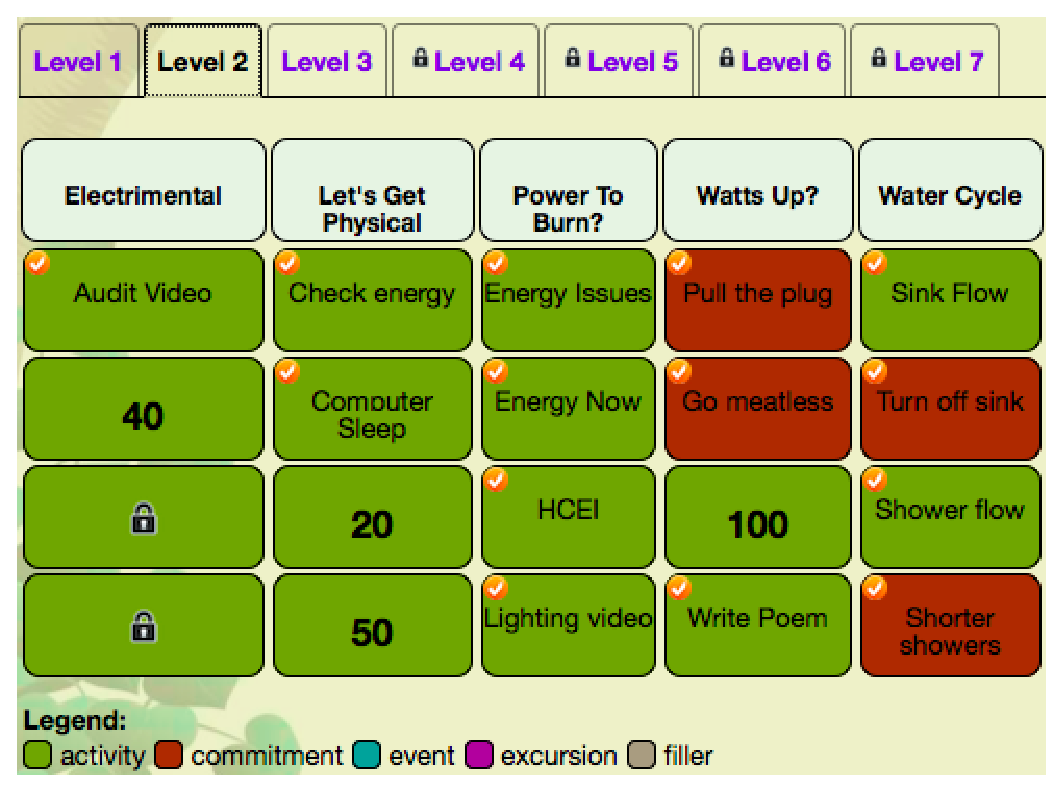
\includegraphics[width=0.95\columnwidth]{smart-grid2.eps}
	\caption{The Smart Grid Game widget, displaying the actions available in level 2.}
	\label{fig:smart-grid}
\end{figure}

Much of the point competition revolves around a section of the challenge website called the Smart Grid Game (SGG). The Smart Grid Game consists of rows of actions arranged into columns based on a particular topic (similar to the popular game show ``Jeopardy''), shown in \autoref{fig:smart-grid}. Clicking on a square in the SGG shows details about the action and explains how players can complete the action to earn points. There are several types of actions: short YouTube videos on energy and sustainability topics, activities like measuring the flow rate of a shower, excursions such as visiting a farm that produces all its own electricity, and commitments such as carpooling or not eating meat. There are also creative actions such as writing a poem about energy or a letter to the editor on a sustainability topic. The flexibility of the SGG allows us to provide a wide variety of interesting actions for players to take part in.

The completion of each action (with the exception of commitments) is verified through the challenge website before points are awarded. For activities, players are usually asked a randomly-selected question, and their answer is placed in a queue for challenge administrators to review. The administrator can approve or reject the submission, and can provide feedback on the player's answer. The game also supports activities that are verified by submission of an uploaded image such as a photo or screenshot.

To encourage players to interact with each other during the challenge, the Kukui Cup provides a number of social features. The \emph{social bonus} provides a way for players to earn additional points by completing certain actions with other players. To earn the social bonus, players include the email address of another player when they complete the verification step for an action. If the submitted email address corresponds to a player that has completed that same action, then the submitting player is awarded a small, configurable number of points. In addition to incentivizing joint play, the social bonus can provide a pretext for a player to initiate contact with another player, such as arranging to attend a workshop. In the college residence hall setting, it can be helpful to have such a pretext for meeting new friends. Social media (in particular Facebook) is integrated into the Kukui Cup as well. Players can share their game accomplishments directly on Facebook, and the Kukui Cup Facebook page is used to share information about the challenge, including upcoming events and short videos of events that have taken place.

As part of the initial log on process to the Kukui Cup website, new players can enter in the email address of a referring player to earn a \emph{referral bonus}. To ensure that the new player starts actually playing the game, they must earn a certain number of points before both the referred and referring player receive the referral bonus points. In the 2012 Kukui Cups, the referral bonus is variable based on the degree of the new player's team participation, so more bonus points are received if the new player is from a team with few participants. The variable referral bonus encourages players to reach out to teams that are not yet involved in the Kukui Cup and gives a small boost to those new players.

Kukui Cup challenges can also be configured to provide incentives to players in the form of prizes for the top scores both at the individual (points) and team level (points and energy use). One problem with the prizes provided in the competition as incentives is that they only go to the top performers in each competition. For those participants so far behind the leaders that they know they will not win the point competitions, the prizes provide little incentive, or possibly a disincentive: why play if there is no way to win a prize? Another problem with the prizes is that to be effective they had to appeal to all participants, limiting the options for prizes.

We developed the Raffle Game to provide a prize-based incentive to play that was not limited to the top players, through inspiration from Prabhakar's work incentivizing road congestion reduction~\cite{Merugu2009}. In the Raffle Game, there are a variety of raffle prizes available in each round of the competition. For each 25 points a participant earns, they receive a virtual raffle ticket. Participants can allocate their raffle tickets among the prizes available, and they can change their allocations at any time until the end of the round. Then a winning ticket is ``drawn'' from those allocated to each raffle prize, and the owner of that ticket wins the prize.

\subsection{Running a Kukui Cup}

A Kukui Cup challenge consists of multiple components working together to provide the entire game experience. For challenges using real-time energy data, the open source WattDepot~\cite{csdl2-10-05} system is used to collect, store, and analyze the data. The challenge website and associated game mechanics are provided by the open source Makahiki system~\cite{csdl2-11-07}. The current educational content is tailored to the needs of college students living in residence halls in \Hawaii, but can be tailored or replaced to suit the needs of other contexts.

The final component in a Kukui Cup challenge are the administrators. Challenge administrators need to plan out the parameters of the competition (duration, number of teams), make game design choices such as point rubrics, customize the educational content for their organization, organize workshops, review player verification submissions, and distribute prizes. Kukui Cup challenges are labor intensive, but that labor provides the opportunity to interact with the players more fully and provide them with a expansive game experience.

\subsection{Field Studies}

In addition to in-lab evaluations and beta tests, there have been two sets of field studies of Kukui Cup challenges. The first Kukui Cup challenge took place over 3 weeks starting in October 2011 in four residence halls for first-year students on the University of \Hawaii at \Manoa campus containing a total of approximately 1070 residents. Each residence hall was further broken into five pairs of floors, each of which share a common lounge area. These pairs of floors are referred to as \emph{lounges}, and were the team unit in the 2011 Kukui Cup.

The second set of challenges started in September 2012. The University of \Hawaii (UH) Kukui Cup is taking place in the same four residence halls with approximately the same number of residents. However, instead of three weeks, the 2012 UH Kukui Cup will take place over nine months of the academic year. The first month of the competition will be an intensive period with multiple real-world events taking place each week, while the remaining months will be less intensive. The goal of the much longer time frame is to discourage short-term and unsustainable behaviors (such as forgoing all electronic device use). 

In addition to the 2012 UH Kukui Cup, Hawaii Pacific University (approximately 200 residents) and the East-West Center (approximately 130 residents) are also running their own challenges using the Kukui Cup system with our support.

\section{Baselines and Goals}
\label{sec:goals-baselines}

Goals have been shown to be effective tools in changing energy consumption behavior~\cite{Becker78, Houwelingen89} and are a common component of eco-feedback mechanisms. Setting achievable goals is important from a gameplay perspective, so goals must typically be based on previous energy use. The most common way to generate a goal is to calculate a \emph{baseline} of energy usage based on past energy usage, and then set the goal as some percentage reduction from the baseline.

Two of the most common ways to calculate the electricity baseline are to average recent prior usage (such as the last two weeks), or to average usage from previous years. Both of these methods are problematic because they assume that this previous usage is representative of future usage, even though there are many factors that can significantly alter electricity use over time including: occupancy, weather, activities (e.g., studying for a big midterm exam), and changes to the building infrastructure such as efficiency upgrades. Any of these factors can lead to the baseline being an inaccurate predictor of future usage in an energy competition, as described by Johnson et al.~\cite{csdl2-12-08}.

Since baselines can be poor predictors of future electricity use, comparing actual electricity use to the baseline in order to determine how much electricity was ``saved'' by an intervention is misleading and can tempt designers to make claims about energy saved that cannot be substantiated. However, comparison of actual electricity usage to a goal generated from a baseline can be helpful as a game mechanic to motivate players to conserve energy.

In the 2011 Kukui Cup, we used a baseline that was derived from an average of the two weeks prior to the challenge. In the 2012 Kukui Cups, we have switched to a dynamic baseline~\cite{csdl2-12-08} that consists of the average electricity usage for the two previous weeks, but the baseline is recomputed every day throughout the challenge. The dynamic baseline means that as the challenge progresses, the baseline will include usage during the challenge. In essence, a goal generated from a dynamic baseline requires a team to reduce their energy usage compared to the recent past. Since the baseline is not a static value picked once before the challenge, anomalous conditions during the period before the challenge will soon be replaced with new, more representative data.

We incorporate the energy goal into an eco-feedback game called the Daily Energy Goal Game (DEGG). Each team has a daily energy goal determined by the baseline. When a team's energy usage at the end of the day is equal to or below the goal, they win the DEGG for that day. In the 2012 Kukui Cups, the energy competition is scored by the number of daily energy goals that each team has achieved, rather than an absolute measure of how much energy has been used or how much a team has reduced their usage below the baseline. By counting goals rather than measures of absolute or relative energy reductions, we hope to incentivize sustainable longer-term behavior changes rather than radical short-term changes such as moving out of the residence hall and into tents (as has been reported anecdotally in some other energy competitions). In an effort to link the energy and point competitions, when a team meets their daily energy goal, each team member receives a configurable number of points.


\section{Eco-Feedback Design Experiences}

\begin{figure}[!tb]
	\centering
	\includegraphics[width=0.7\columnwidth]{energy-24hours-new.eps}
	\caption{A bar chart visualization of energy use as compared to a goal over 24 hours}
	\label{fig:energy-24hours}
\end{figure}

Feedback on electricity consumption has been used as a means for facilitating energy conservation by researchers in the CHI community~\cite{Froehlich2010} as well as in the broader energy efficiency~\cite{darby-review-2006, Faruqui09, Foster-2012} and environmental psychology~\cite{Becker78, Houwelingen89} communities. One reason for this focus on feedback is undoubtedly the hidden nature of electricity, so feedback provides an awareness that is otherwise unavailable.

One of the fundamental principles of eco-feedback in the Kukui Cup is that it be \emph{actionable}. We feel strongly that eco-feedback that does not guide viewers towards actions that they can take will be ineffective in achieving our goal of providing insight into energy-related behaviors. While any energy feedback may implicitly encourage energy conservation behaviors simply by making energy use visible, this does not meet our definition of actionable. A feedback display that shows that a home has used 20 kWh so far on a particular day leaves the viewer with natural questions: is that a lot? what should I do if I wanted to reduce my energy use?


\subsection{The Eco-Bar Chart Visualization}


An early attempt at eco-feedback for the Kukui Cup is shown in~\autoref{fig:energy-24hours}. This ``Eco-Bar Chart'' shows hourly energy use for a team participating in the Kukui Cup over 24 hours as compared to an energy goal. Note that the data shown in this particular figure are simulated. Bars that are entirely green show the actual energy usage for that hour and indicate that the energy use was below the hourly goal. For mixed red and green bars, the main green portion represents the energy goal for that hour of the day, while the red tips of the bars represent the actual usage in excess of the goal.

This form of eco-feedback shows the variation in energy use over the course of a day, which is an important energy literacy concept. It also shows in what parts of the day energy use is exceeding the goal, and by how much. By displaying the times during the day when the hourly goals are not being met, residents could focus on understanding what activities are going on during those periods.

As (naive) designers, we felt that this eco-feedback provided a great deal of useful feedback both clearly and concisely. However, results of an in-lab evaluation were unequivocal: the visualization provided too much information, the meaning of its components was not obvious, and the ``actionable'' aspects were not obvious. This eco-feedback was a failure, and we began a redesign to address its deficiencies.

\subsection{The Power Meter Eco-Feedback Visualization}

\begin{figure}[!tb]
	\centering
	\includegraphics[width=0.65\columnwidth]{power-meter.eps}
	\caption{The Power Meter eco-feedback visualization}
	\label{fig:power-meter}
\end{figure}

Another early eco-feedback visualization developed for the Kukui Cup is the Power Meter, shown in \autoref{fig:power-meter}. The Power Meter is an example of one of the most common types of eco-feedback visualizations: a near real-time representation of how much power is being used. In the UH Kukui Cup, the Power Meter reflects the power use of a lounge consisting of 54 residents. The meter is calibrated so that the middle reading (needle pointing straight up) corresponds to the average team power use computed from the hourly baseline data, and the range of the meter dial is set to account for the largest swings in power use based on historical data. This calibration means that if the needle is on the right side of the dial it reflects more team power use than ``normal'' for this hour and day, and conversely if the needle is on the left side, it corresponds to less power usage than normal. The calibration is updated each hour to match the new hourly baseline.

The motivation for the Power Meter was to enable players to explore their power use in real time by turning devices around their room and floor on and off to see how it impacted their power use, a classic use of high-frequency feedback. However, we have seen no evidence, anecdotal or otherwise, that players have actually used the Power Meter visualization in this way. One difference between the Power Meter as used in the UH Kukui Cup challenges and similar eco-feedback devices in a home setting is that there are many more people living in the metered space in the UH Kukui Cup. The large number of people whose electricity use is being metered makes it more difficult to see changes due to an individual device, unless that device uses a large amount of power (such as a microwave or hair dryer). The Power Meter eco-feedback visualization was, therefore, a failure with respect to the use we intended. However, we have left the Power Meter as part of all Kukui Cups using real-time meter data as a counterpoint to the energy-based Daily Energy Goal Game visualization in the hope of reinforcing the difference between power and energy.

\subsection{The Daily Energy Goal Game Eco-Feedback Visualization}

\begin{figure}[!tb]
	\centering
	\includegraphics[width=0.95\columnwidth]{degg.eps}
	\caption{The Daily Energy Goal Game eco-feedback visualization}
	\label{fig:degg}
\end{figure}

To make our eco-feedback easier to understand and also more actionable, we developed the Daily Energy Goal Game (DEGG) visualization shown in~\autoref{fig:degg}. The three most prominent components of the DEGG are: the energy consumption so far during the current day, the energy goal so far for the current day, and a traffic light that shows in the most straightforward way whether the team is meeting their energy goal. The display updates once every 10 minutes with new energy data.

We picked the daily time frame for the game for two reasons. First, having a daily goal makes behavior changes more visible and feedback more immediate than a longer time frame such as weekly or monthly. Second, by concentrating on a daily goal, teams that are performing poorly on a particular day can redouble their efforts to do better the next day. Similarly, a team that does particularly well for one day cannot rest on their laurels, they must make an effort to conserve on every day. This game design reflects our belief that changing energy behaviors is a marathon and not a sprint: radical short-term changes made to win an energy competition are unlikely to be sustainable, and are therefore of very limited utility.

Residential energy use varies in intensity over the course of a day: typically low when people are sleeping and much higher during evening hours. For the students in the residence halls in our studies, the energy usage peak occurs at approximately midnight, and the lowest value is between 8 and 9 AM, which is considerably different than an average single-family home. There is also daily variation between days of the week, as the activities taking place on a Monday night are different than those on a Saturday night. To account for the hourly and daily variation in energy use, our we compute hourly and daily baselines for energy use, and the goal value is a percentage reduction from the baseline. The energy consumption and goal values displayed in the DEGG are computed over the time period from midnight to the current time. This choice of time frame is particularly important for the goal value, because if a daily goal value was simply spread linearly over the course of a day, players would see their energy use as always under the goal during low-usage periods, but then going above the goal during the high-usage periods, possibly to a degree that makes it impossible to meet the goal for that day.

Below the traffic light display of the DEGG is a list of actions from the Smart Grid Game that players can take to either learn more about energy, or directly help reduce their energy use. The actions displayed depend on what actions the player has already completed in the rest of the system. The direct links to actions that players can take to reduce their energy usage, tailored to the opportunities available in their residence hall make the DEGG highly actionable.

Evaluation of the DEGG visualization during actual game play indicates that players do not have a problem understanding the visualization. The stoplight image provides a clear, unambiguous signal, and the actual/goal numbers provide further context. In addition, the visualization is explicitly paired with links to descriptions of appropriate actions for that player in the context of the game and the team's current energy use. Log data indicates that players do click on these links in order to understand how to take action based on the eco-feedback. This eco-feedback was a success and is included in the current version of the Kukui Cup.

%% Add section on manual energy data DEGG?

\subsection{The ``Wii Hours'' Eco-Feedback Visualization}

\begin{figure}[!tb]
	\centering
	
\includegraphics[width=0.6\columnwidth]{how-meet-goal.eps}
	\caption{The ``How can we make our daily goal?'' widget}
	\label{fig:make-goal}
\end{figure}

In another eco-feedback design effort, we created a small widget below the DEGG titled ``How can we make our daily goal?''. This widget, shown in~\autoref{fig:make-goal}, showed how much the player's team energy usage was above the goal, and provided a drop-down menu of electrical devices commonly present in student rooms: laptops, XBox 360, Wii, etc. When a device was selected from the menu, the system would display the approximate number of hours of device use that would equal the amount of team energy use over the goal value. The time value was intended to show players how much device use they would need to \emph{forego} in order to get back on track to their energy goal, and develop their intuition about the relative power use of different devices (i.e., plasma TVs use much more power than Wii game consoles). Therefore a short time value could point out an easy way to make the goal, and a long time value would indicate less significant energy conservation.

However, during in-lab evaluations of the system, we found that multiple subjects misinterpreted the time value, thinking that high time values were bad rather than good. Since the Wii was the device on the list with the smallest power use (20 W) compared to an XBox 360 or Playstation 3, it led to the highest time values. Some subjects drew the conclusion that using a Wii was worse than using an XBox 360 or Playstation 3, which was precisely the opposite goal of this widget. One subject even took the time to use our in-game team discussion forum to post the message ``don't play wii'' after using the widget! Because of this example, we dubbed this confusion the ``Wii problem''.

Clearly, eco-feedback that can lead at least some players to the opposite conclusion than intended is a failure. The ``Wii Hours'' visualization never made it into production, and we are still searching for a design variant that can convey this information in an unambiguous fashion to players with minimal energy literacy.


\subsection{Canopy Eco-Feedback}

The 2011 Kukui Cup took place over three weeks, and as part of the game experience we wanted to create a more advanced level of experience for the top participants in the competition. The background of the competition website featured a forest theme, so the Canopy was named to convey that it existed ``above'' the rest of the website. The Canopy was conceived as a way to keep the top participants engaged even if they had completed most of the activities available in the Smart Grid Game. A primary way to accomplish this was the use of more sophisticated visualizations that would demand more thought from the top players. 

The Canopy provided a series of ``missions'' that players could undertake. Some Canopy missions were to be accomplished individually, while other missions required 2 or 3 participants to work together. Players could indicate that they were ``up'' for a group mission to find other interested participants. Missions included looking at more advanced energy visualizations, and also activities such as seeking out places on campus that are wasting energy.

Canopy missions were like activities available in the rest of the game, but instead of earning points upon completion, Canopy activities earned \emph{Canopy Karma}, which was a separate point system for the Canopy. Canopy Karma was used instead of the standard points to ensure that the Canopy itself did not unbalance the point competition by providing a way for the top players to earn more points that were not available to the rest of the participants.

The energy data and visualizations available in the forest, such as the Daily Energy Goal Game described above, were deliberately simple to avoid confusing participants with low energy literacy. The requirement for simplicity meant the energy data shown to players comes only from the participant's team. This constraint could be relaxed in the Canopy, as users were more sophisticated and presumed interested in comparative and other analyses.

\begin{figure}[!tb]
	\centering
	\includegraphics[width=0.95\columnwidth]{hot-spots-crop2.eps}
	\caption{Example canopy eco-feedback: Energy Hot Spots}
	\label{fig:hot-spots}
\end{figure}

\autoref{fig:hot-spots} shows ``Energy Hot Spots'', one of several forms of advanced eco-feedback made available in the Canopy. This visualization shows hourly electricity use for a selected team over the course of a selected week. This breakdown allows players to examine their usage patterns and see how they change throughout the day, between days of the week, and between different teams. The Canopy mission based around the Energy Hot Spots eco-feedback asked players the following questions:

\begin{itemize}
	\item What hours of the day seem to have the highest energy use? How does that compare to your own energy use patterns?
	\item What differences in energy use do you notice between teams?
	\item What are your thoughts on this visualization? What are its strengths and weaknesses?
\end{itemize}

The Canopy was introduced in the third week of the 2011 Kukui Cup, and the top 42 players were invited to enter the Canopy out of a total of 401 players. Although use of the Canopy was quite limited, players' feedback about these advanced forms of eco-feedback was uniformly positive: they reported enjoying the ability to compare energy use between teams and seeing what times different teams energy use peaked. 

This positive feedback indicates that the Canopy eco-feedback was a success, and also indicates the critical role of context and scaffolding in eco-feedback design. 


\section{Domain Knowledge and Eco-Feedback}

Eco-feedback systems provide data on some aspect of behavior with the goal of reducing negative environmental impact~\cite{Froehlich2010}. However, they often assume users possess some level of domain knowledge about the environmental topic they hope to address. In the area of energy, the term \emph{energy literacy} has been used to describe the understanding of energy concepts as they relate both on the individual level and on the national/global level.

Some examples of energy literacy are:

\begin{itemize}
	\item Understanding the difference between power and energy;
	\item Knowing that a microwave uses much more power than a refrigerator, but that the refrigerator will use much more energy over time; and
	\item Knowing how electricity is generated in one's community.
\end{itemize}

Unfortunately, all indications are that energy literacy is low in the United States. DeWaters and Powers have developed an energy literacy survey instrument for middle and high school students~\cite{DeWaters2007,DeWaters2008}. They found that the student mean attitude scores were 73\%, but that knowledge scores lagged far behind (42\% correct)~\cite{DeWaters2011}. Based on their findings, they make some recommendations, such as energy curricula be ``hands on, inquiry based, experiential, engaging, and real-world problem solving \ldots'', and using the campus as a ``learning laboratory''. Similarly a nationwide survey of adults on energy by Southwell et al. found that the average respondent answered fewer than 60\% of the energy knowledge questions correctly~\cite{Southwell2012}.

One energy literacy topic that we emphasize in the Kukui Cup is the difference between power and energy, power being the rate at which energy is being consumed or produced (measured in watts) and energy is the quantity of work that can be performed by a system (measured somewhat confusingly for electricity in kilowatt-hours). In the Kukui Cup we explain this relationship as being analogous to speedometer and odometer in a car.

Through answers submitted to the online activities in the Kukui Cup, we can see that many players have trouble understanding the concepts of power, energy and their interrelationship. Players often confuse the two concepts and often fail to grasp the time sensitivity of power, and thereby considering devices that consume a lot of power as ``bad'' irrespective of how long they are actually used. When the users of visualizations do not understand the concepts that are being visualized, understanding of the visualizations becomes much more difficult. It is for this reason that we claim that eco-feedback systems should incorporate educational components, or risk being unintelligible to users. However, we reject the notion that power and energy, watts and kilowatt-hours are too complicated and that users should be provided instead with analogies to cars driven or hamburgers eaten. These energy concepts are important for our energy future, and should not be reduced to analogies alone.

% Short answer questions can prompt players to reflect on their experiences

\subsection{Moving Beyond Individual Actions}

In addition to shorter activities available in the SGG, the Kukui Cup also provides creative activities to encourage more in-depth explorations of energy and sustainability. These creative activities run the gamut from writing a haiku about a sustainability topic, to conducting an interview, or making a video. Creative activity submissions from players are assigned a point value by administrators based on the quality of the work and the effort required to make. We hope that the creative activities provide a different outlet for players, and encourage them to think beyond their individual actions and bring a sense of ownership to the cause of sustainability.

As mentioned previously, the 2012 UH Kukui Cup will run for an entire academic year. Much of the educational content we have developed will be made available to players in the first intensive month of the challenge, leaving later rounds with less content, and thereby fewer reasons to continue playing. To address this problem, and to draw players into deeper play and understanding of sustainability issues, players will be able to suggest new additions to the SGG as part of the game. Players that provide useful new activities and events for the the game will earn points, and once the new actions are placed into the SGG, they will have provided additional educational content for other players. We are also exploring ways to tie class work into the Kukui Cup challenge. With the longer time frame afforded by the nine month competition, we intend to allow players to earn points in the competition by registering for sustainability-related classes, and picking sustainability-themed class projects. Ultimately, we hope the Kukui Cup will lead to macro behavior changes like selecting a sustainability degree program or choosing a more efficient vehicle.

We have also witnessed improvements in players' energy literacy in the course of a single workshop. In the energy scavenger hunt workshop, attendees are grouped into teams of 3--4 people and provided with a plug load meter that shows the amount of electrical power consumed by whatever device is plugged into the meter. Each team is given 30 minutes record the power use of devices in their rooms and residence halls, looking for devices with the highest power use they can find, and also the most number of devices with distinct power use in 10\,W intervals. The goals of the workshop (beyond entertainment) are to train players to measure device power use, and also to build their intuition about how much power different devices use. In the 2011 Kukui Cup, after the teams completed their hunt, each team was asked to present their results. One team reported that the microwave they measured used 200\,W, and immediately several players from other teams shouted out that the first team must have done something wrong because microwaves use over 1000\,W, as they started to form their energy intuition based on their own hunt.

There is a proposed renewable energy project in Hawaii called ``Big Wind'' that would generate as much as 400\,MW of electricity from wind farms covering substantial portions of two more rural islands (Moloka`i and L\=ana`i) with excellent wind resources. The power would be transmitted via a new undersea cable to O`ahu, which has the majority of the state's population, but with inferior wind resources. There are advocates both for and against Big Wind, but to make an informed decision one should understand how O`ahu's electricity is generated now, and the characteristics and challenges of wind energy. We hope that the educational activities that are part of the Kukui Cup will equip players to make informed choices on these types of thorny policy questions.


\section{Eco-Feedback, Stickiness, and Serious Games}

A meta issue for all eco-feedback systems is how to ensure that they continue to be ``sticky'' for users, as a feedback system that users do not look at will be unable to accomplish anything. There are indications that the long-term impact of eco-feedback may be diminished due to habituation. Froehlich suggests that the average user will spend less than one minute per day exploring their energy consumption behaviors~\cite{Froehlich2010-BECC}. A study by Houde et al. of households using Google PowerMeter found an ``immediate decrease in electricity consumption, but in the long term these electricity savings decrease and disappear.''~\cite{Houde2013-powermeter} This finding suggests that a primary concern for any eco-feedback system is ensuring that users continue to interact with it over the long term. Put another way, eco-feedback alone is not enough to accomplish the goals that most eco-feedback systems hope to achieve.

One solution to the lack of stickiness of eco-feedback systems is the incorporation of game play. Serious games like the Kukui Cup provide an alternative route to promote both learning and engagement with energy feedback. It is for this reason that we designed the Kukui Cup as a serious game that incorporates electricity consumption feedback as one aspect of the game experience, rather than an eco-feedback system that has been ``gamified''. 

One issue with the Kukui Cup is that the educational content is largely of interest only until its content has been assimilated. We do not anticipate that players would want to revisit most actions unless they were able to earn additional points. This limited engagement is in contrast to games that players enjoy playing over and over. Some serious games such as the protein folding game Foldit do manage to attract repeat players and meet their serious goals~\cite{Khatib2011}. While the Kukui Cup may stop being of interest to players once they have completed all the content available, we hope that our attempts to engage players in broader sustainability opportunities such as taking classes and becoming involved in campus and community organizations make the Kukui Cup no longer necessary for them.

While games are not the only way to promote long-term engagement with energy issues, we submit that any normal eco-feedback system will quickly be abandoned by users once the novelty wears off. There must be a continuing reason for users to revisit the system that even the most novel and interesting eco-feedback systems lack.


\section{Discussion}

We now return to the three survey papers mentioned in the introduction to see how their recommendations for eco-feedback systems relate to our experiences with the Kukui Cup. The recommendations from Froehlich et al.~\cite{Froehlich2010} match up well with our research. The Kukui Cup is grounded in the extensive work from the environmental psychology, popularized by the Community-Based Social Marketing (CBSM) process~\cite{McKenzie-Mohr2009} including goal setting and public commitments. The Kukui Cup goes beyond the smaller-scale evaluations of many eco-feedback systems, engaging hundreds of players at multiple institutions. The 2012 UH Kukui Cup will run for nine months, far longer than the evaluation of most eco-feedback systems. Froehlich et al. also point out that most eco-feedback systems focus on curtailment behaviors (such as turning off lights when leaving a room) at the expense of efficiency behaviors (such as installing more efficient light bulbs), despite evidence that efficiency behaviors might be much more effective. While a significant portion of the Kukui Cup focuses on curtailment behaviors, there are a number of activities that focus on efficiency behaviors such as replacing an incandescent light bulb with a compact fluorescent lamp, and exploring the relative efficiencies of different  vehicles. Froehlich et al. also point towards learning as an important area for eco-feedback research, and educational content is an essential part of the Kukui Cup experience. Finally, Froehlich et al. suggest that large scale commercial deployments of eco-feedback technology may produce interesting results. While the Kukui Cup has not been deployed at a large commercial scale, it is based on open source software and freely-redistributable content, allowing others to deploy their own Kukui Cup challenges. Interestingly, both systems mentioned by Froehlich et al. as potential large-scale deployments (Google PowerMeter and Microsoft Hohm) have been discontinued, which is not a problem for systems based on freely-available components.

One recommendation from Pierce and Paulos~\cite{Pierce2012-BEM} is the use of ``energy metadata'' to tag energy with characteristics such as how it was produced. While the Kukui Cup does not provide any metadata, it is highly concerned with the issue of how energy is generated, with a significant portion of the educational content focused on how \Hawaii generates its energy. Brynjarsd\'{o}ttir et al. suggest that persuasive sustainability systems should include users in the design process. In the Kukui Cup, it is not generally feasible to include the actual players into the design process since that design process took place long before the players reach campus. The Kukui Cup team includes undergraduates who have lived in the residence halls, and we have recruited 2011 UH Kukui Cup players to assist in the planning of the 2012 UH Kukui Cup. As discussed earlier, the 2012 UH Kukui Cup also provides a way for players to earn points for suggesting new activities and organizing events, which is a simple form of in-game participatory design.

Both Pierce and Paulos and Brynjarsd\'{o}ttir et al. suggest eco-feedback or persuasive sustainability systems need to move beyond their current focus on the individual, and engage users on the complex and less easily measured aspects of sustainability such as community and political issues. The Kukui Cup attempts to take on this challenging issue through the creative, open-ended activities made available to players such as interviewing relevant policymakers, and providing points for attending events held by campus and community environmental organizations.


\section{Future Work}

The Kukui Cup is an ongoing project and we continue to build upon our initial work. The first area of future work is the 2012 UH Kukui Cup. The 2012 UH Kukui Cup will last nine months and should shed light on several issues: can we  maintain player interest over longer periods despite fewer prompts from intensive marketing and events, can the new player-provided educational content fill the gap of the longer challenge duration, and the results of the DEGG with dynamic baselines over a long time frame.

The 2012 Kukui Cups happening at Hawaii Pacific University and the East-West Center will also offer new insights into how challenge administrators outside our research group design Kukui Cup challenges tailored to their organization, and how different student populations perform in the Kukui Cup.

Beyond college campuses, we are considering expanding the Kukui Cup to other organizations in \Hawaii including middle and high schools. Kukui Cups run in schools will require changes to the educational content to make it more relevant to those students, but may provide opportunities for integrating into the curriculum.

We hope one day to be able to run a Kukui Cup challenge that anyone in the State of \Hawaii can participate in. The Kukui Cup is currently a effort-intensive program, so scaling to hundreds of thousands of players will require scaling the management of the challenge, finding a means of funding, and a way for players to incorporate household energy data fairly in a completely heterogenous environment.

One final area of research is longitudinal studies of players after the game is over and they have moved out of the residence halls. We want to find out whether the Kukui Cup experience actually had lasting impacts on players, and whether they were able to continue any new behaviors after leaving the context of the residence hall.


\section{Conclusion}

We have described the Kukui Cup serious game, and our results from field trials of the system. We have discussed some of the eco-feedback visualizations we developed, including both those that succeeded and those that failed. Based on our experiences, we provide three areas that eco-feedback systems should address: they should be actionable, they must address users lack of domain knowledge, and they must find ways to be sticky. We have also shown how the Kukui Cup research can address some of the critiques of eco-feedback systems described in the literature.


\section{Acknowledgments}

Omitted from review version.

%\textbf{Don't forget
%to acknowledge funding sources as well}, so you don't wind up
%having to correct it later.

% Balancing columns in a ref list is a bit of a pain because you
% either use a hack like flushend or balance, or manually insert
% a column break.  http://www.tex.ac.uk/cgi-bin/texfaq2html?label=balance
% multicols doesn't work because we're already in two-column mode,
% and flushend isn't awesome, so I choose balance.  See this
% for more info: http://cs.brown.edu/system/software/latex/doc/balance.pdf
%
% Note that in a perfect world balance wants to be in the first
% column of the last page.
%
% If balance doesn't work for you, you can remove that and
% hard-code a column break into the bbl file right before you
% submit:
%
% http://stackoverflow.com/questions/2149854/how-to-manually-equalize-columns-
% in-an-ieee-paper-if-using-bibtex
%
% Or, just remove \balance and give up on balancing the last page.
%
\balance

% If you want to use smaller typesetting for the reference list,
% uncomment the following line:
% \small
\bibliographystyle{acm-sigchi}
\bibliography{sustainability,csdl-trs,gamification}
\end{document}
